%%%%%%%%%%%%%%%%%%%%%%%%%%%%%%%%%%%%%%%%%
% Journal Article
% LaTeX Template
% Version 1.2 (15/5/13)
%
% This template has been downloaded from:
% http://www.LaTeXTemplates.com
%
% Original author:
% Frits Wenneker (http://www.howtotex.com)
%
% License:
% CC BY-NC-SA 3.0 (http://creativecommons.org/licenses/by-nc-sa/3.0/)
%
%%%%%%%%%%%%%%%%%%%%%%%%%%%%%%%%%%%%%%%%%

%----------------------------------------------------------------------------------------
%	PACKAGES AND OTHER DOCUMENT CONFIGURATIONS
%----------------------------------------------------------------------------------------

\documentclass[twoside]{article}

\usepackage[utf8]{inputenc}
\usepackage[ngerman]{babel}

\usepackage[sc]{mathpazo} % Use the Palatino font
\usepackage[T1]{fontenc} % Use 8-bit encoding that has 256 glyphs
\linespread{1.05} % Line spacing - Palatino needs more space between lines
\usepackage{microtype} % Slightly tweak font spacing for aesthetics

\usepackage[hmarginratio=1:1,top=32mm,columnsep=20pt]{geometry} % Document margins
\usepackage{multicol} % Used for the two-column layout of the document
\usepackage[hang, small,labelfont=bf,up,textfont=it,up]{caption} % Custom captions under/above floats in tables or figures
\usepackage{booktabs} % Horizontal rules in tables
\usepackage{float} % Required for tables and figures in the multi-column environment - they need to be placed in specific locations with the [H] (e.g. \begin{table}[H])
\usepackage{hyperref} % For hyperlinks in the PDF
\hypersetup{%
  colorlinks   = true, %Colours links instead of ugly boxes
  breaklinks   = true,
  urlcolor     = blue, %Colour for external hyperlinks
  linkcolor    = blue, %Colour of internal links
  citecolor    = black %Colour of citations
}
\usepackage[vertfit]{breakurl}

\usepackage{SIunits}

\usepackage{lettrine} % The lettrine is the first enlarged letter at the beginning of the text
\usepackage{paralist} % Used for the compactitem environment which makes bullet points with less space between them

\usepackage{wasysym}
\usepackage{marvosym}

\usepackage{apacite}

\usepackage{abstract} % Allows abstract customization
\renewcommand{\abstractnamefont}{\normalfont\bfseries} % Set the "Abstract" text to bold
\renewcommand{\abstracttextfont}{\normalfont\small\itshape} % Set the abstract itself to small italic text

\usepackage{titlesec} % Allows customization of titles
\renewcommand\thesection{\Roman{section}}
\titleformat{\section}[block]{\large\scshape\centering}{\thesection.}{1em}{} % Change the look of the section titles

\usepackage{graphicx}
\usepackage{pstricks}
\usepackage{pstricks-add}
\usepackage{pst-barcode}
\usepackage{pst-bar}
\usepackage{pst-plot}

\usepackage{fancyhdr} % Headers and footers
\pagestyle{fancy} % All pages have headers and footers
\fancyhead{} % Blank out the default header
\fancyfoot{} % Blank out the default footer
\fancyhead[C]{Scientifica Ambulo $\bullet$ Juli 2013 $\bullet$ Vol. I, No. 1} % Custom header text
\fancyfoot[RO,LE]{\thepage} % Custom footer text

\usepackage[ngerman]{cleveref}


%----------------------------------------------------------------------------------------
%	TITLE SECTION
%----------------------------------------------------------------------------------------

\title{\vspace{-15mm}\fontsize{24pt}{10pt}\selectfont\textbf{Die Ötschergräben}} % Article title

\author{%
Michael Fladischer
\and
Martina Schlaipfer
\and
Matthias Schlaipfer
\vspace{-5mm}
}
\date{}

%----------------------------------------------------------------------------------------

\begin{document}

\maketitle % Insert title

\thispagestyle{fancy} % All pages have headers and footers

%----------------------------------------------------------------------------------------
%	ABSTRACT
%----------------------------------------------------------------------------------------

\begin{abstract}

\noindent Dies ist eine Einladung zu einer Wanderung in den wunderbaren
Ötschergräben, dem ``Grand Canyon Österreichs''. Ähnlich wie im Vorjahr wollen
wir wieder die Wege entlang des erfrischenden Ötscherbaches unsicher machen.
Dieses Dokument soll sowohl der Schmackhaftmachung, als auch der Organisation
dieses Pflichttermins dienen.

\end{abstract}

%----------------------------------------------------------------------------------------
%	ARTICLE CONTENTS
%----------------------------------------------------------------------------------------

\begin{multicols}{2} % Two-column layout throughout the main article text

\section{Einleitung}

\lettrine[nindent=0em,lines=3]{I} m Volksmund auch als der ``Grand Canyon Österreichs'' bezeichnet, liegen die Ötschergräben südlich am Fuße des
Ötscher-Gebirgsmassivs. Der sechs Kilometer lange Graben wird vom Ötscherbach durchzogen, der auf einer Höhe von ca. 1100 Meter über dem Meeresspiegel
entspringt. Bekannt für ihr klares Wasser und die Wasserfälle, die entlang des Ötscherbaches in den Graben stürzen, sind die Ötschergräben ein beliebtes
Ausflugsziel für Wanderer.

Das Ötscher-Gebirgsmassiv wird geologisch dem Alpenvorland als Teil der Kalkalpen zugerechnet. Zusammen mit dem Schneeberg und dem Wiener Becken bildet es die
Kalkvoralpen. \cite{SH:2012}

Geographisch liegt das Gebirge im Gebiet des Naturparks Ötscher-Tormäuer, welcher 1970 als Folge einer Protestbewegung gegen ein neues Wasserkraftwerk an der
Erlauf entstand \cite{NOT:2013:Online}. Das Gebiet um den Naturpark ist vor allem seit der Zuwanderung eines Bärenmännchens aus Slowenien Anfang der 1970er
Jahre und der darauf folgenden Ansiedelung von drei weiteren Bären in den nördlichen Kalkalpen bekannt.

Im Sommer des Jahres 2012 unternahmen kälteresistente Mitglieder (\cref{fig:bad}) der bergbegeisterten Familie Maierhofer gleich zwei Wanderungen, welche auch
ein Bad in den Bächen abseits der Wanderwege einschloß. Dies waren zuerst in der Bärenschützklamm und dann, im größeren Rahmen, in den Ötschergräben, nahe den
Mirafällen.

Aufgrund der Begeisterung einer representativen Population der Teilnehmer aus dem Jahr 2012 soll auch heuer wieder eine Wanderung in das Gebiet der
Ötschergräben unter möglichst umfassender Beteiligung aller Familienmitglieder stattfinden.

\begin{figure}[H]
\begin{center}
  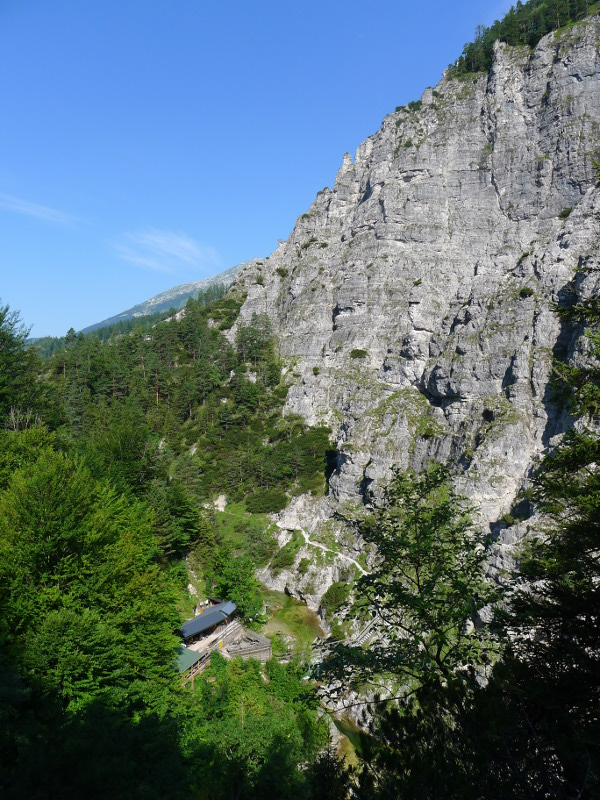
\includegraphics[trim = 0 15 0 0, clip, natwidth=600, natheight=800, width=.45\textwidth]{Figures/oetschergraeben.jpg}
\end{center}
\caption{Schööön!}
\label{fig:oetschergraeben}
\end{figure}

%------------------------------------------------

\section{Ablauf}

\begin{figure*}
\begin{center}
  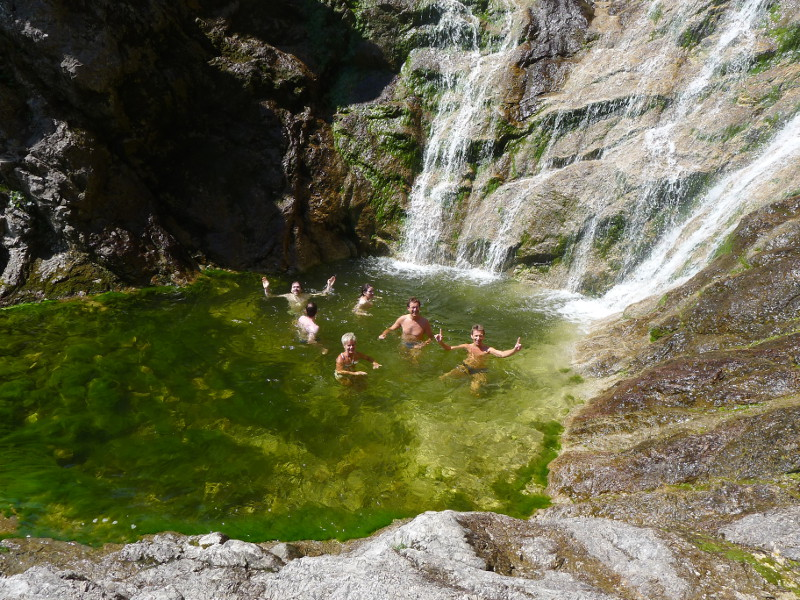
\includegraphics[trim = 0 80 0 80, clip, natwidth=800, natheight=600, width=\textwidth]{Figures/bad.jpg}
\end{center}
\caption{Erfrischend!}
\label{fig:bad}
\end{figure*}

Als Wanderroute für das Jahr 2013 wird eine andere als 2012 vorgeschlagen um eine maximale Erwärmung aller Teilnehmer zu gewährleisten. Ausgangsort für die Tour
ist Mitterbach, nördlich von Mariazell. Der Ausgangszeitpunkt wird wie in \cref{sec:teilnahme} erklärt, bestimmt.

Nach einer Vollständigkeitsprüfung begeben sich die Probanden mit Hilfe des Sessellifts auf die Gemeindealpe wo dann der Fußmarsch beginnt. Das erste Ziel der
Route ist das Gipfelkreuz am "`Eisernen Herrgott"' wo eine Pause eingelegt werden kann, um die Probanden auf erwartete psychologische und körperliche
Effekte des Badens im kalten Wasser des Ötscherbaches zu befragen. Über die Zwischenstation "`Schutzhaus Vorderötscher"' geht es hinab in die Ötschergräben.

Die Route erreicht den Ötscherbach in etwa auf der Höhe der Schleierfälle und ab hier folgt die Route dem Verlauf der Ötschergräben, vorbei an den Mirafällen,
der ersten und bereits bekannten Bademöglichkeit in der Gumpe direkt unter dem Wasserfall. Kurz nach den Mirafällen bietet sich dann die zweite bekannte
Bademöglichkeit, in der besonders tiefen Auswaschung zwischen zwei Gesteinsplatten direkt im Ötscherbach. Nach dieser Station führt die Route weiter talauswärts
zur Jausenstation "`Ötscherhias"' (\cref{fig:oetschergraeben}) wo sich die Probanden wieder erwärmen und stärken können.

Ab diesem Punkt bieten sich zwei Möglichkeiten die Tour zu beenden:

\begin{enumerate}
    \item Wie auch im Jahr 2012, weiter den Ötschergräben folgend in Richtung Wienerbruck. Dabei würde die Route dann auch die im Jahr 2012 erkundete Stelle mit
        dem tief ausgewaschenen Becken unterhalb eines breiten Wasserfalls erreichen, wo sich die letzte Möglicheit zum Baden bieten würde. Weiter geht es dann
        zur Haltestelle Wienerbruck von dort mit der Mariazellerbahn zurück nach Mitterbach.
    \item Ausstieg aus den Ötschergräben hinter dem Ötscherhias, und Zustieg zur Mariazellerbahn bei der Haltstelle Erlaufklause, ebenfalls zurück nach
        Mitterbach.
\end{enumerate}

%------------------------------------------------

\section{Ausrüstung}

\lettrine[nindent=0em,lines=3]{E} ine Wanderung, welche mit einem Bad im Gebirgsbach oder in der Gumpe eines Wasserfalls kombiniert wird, macht es erforderlich,
ein Mindestmaß an empfohlener Ausrüstung mitzuführen. Die folgende Aufzählung sollte als Checkliste während den Vorbereitungen für die Wanderung herangezogen
werden.

\begin{itemize}
    \item[\Square] Badebekleidung (unter der Wanderkleidung oder separat).
    \item[\Square] Trockene Unterwäsche zum Wechseln.
    \item[\Square] Ein oder mehrere Badetücher.
    \item[\Square] Sonnencreme, auch während der Wanderung zu benutzen.
    \item[\Square] Badeschlapfen (optional).
    \item[\Square] Kälteresistenz bis $\unit{283.15}{\kelvin}$.
\end{itemize}

%------------------------------------------------

\section{Teilnahme}
\label{sec:teilnahme}

\lettrine[nindent=0em,lines=3]{D} ie Abstimmung des Termins erfolgt über einen \href{http://www.doodle.com/m6ywebgyvg6632ig}{Doodle}. Smartphone-Benutzer
können den QR-code scannen um auf die entsprechende Seite zu gelangen. Für Benutzer von handelsüblichen PDF-Readern genügt ein Klick auf das blau hervorgehobene
Wort.

Es stehen fünf Termine mit je drei Uhrzeiten zu Auswahl, wobei die Uhrzeit festlegt, wann wir uns in Mitterbach beim Bahnhof treffen.

\begin{figure}[H]
\begin{center}
  
\includegraphics[width=.45\textwidth]{Figures/qr-code.eps}
\end{center}
\caption{Scannen!}
\label{fig:qr-codqr-code}
\end{figure}

%------------------------------------------------

\section{Rückfragen}

\lettrine[nindent=0em,lines=3]{B} ei allfälligen Rückfragen stehen die Autoren selbstverständlich zur Verfügung. Es können auch Kommentare im Doodle
 hinterlassen werden. Sollte es passieren, dass nach der Zusage zu einem Termin dieser doch nicht wahrgenommen werden kann, so bitten wir um kurze Mitteilung.

\begin{tabular}{l l}
\Letter \ \href{mailto:michael@fladi.at}{Michael Fladischer} & \phone \ 0660/4806299 \\
\Letter \ \href{mailto:mschlaipfer@gmx.net}{Martina Schlaipfer} & \phone \ 0680/1302672 \\
\Letter \ \href{mailto:m.schlaipfer@gmail.com}{Matthias Schlaipfer} & \phone \ 0680/2333950 \\
\end{tabular}


%----------------------------------------------------------------------------------------
%	REFERENCE LIST
%----------------------------------------------------------------------------------------

\bibliographystyle{apacite}
\bibliography{literature}

%----------------------------------------------------------------------------------------

\end{multicols}

\end{document}
